\section{联邦学习数据集}
\addcontentsline{toe}{section}{{5.2\ \ Datasets for Federated Learning}\numberline\,}
\label{sec:chap5-datasets}

% NOT finished
% NOT indexed

正如本文\S\ref{sec:chap1-fl-applications}~中提到的,联邦学习所涉及、处理的实际数据往往具有强烈的统计异质性,因此用于联邦学习仿真试验的试验数据集需要以多种方式、从多个角度尽量模拟、贴近这种统计异质性。比较幸运的是,在本章\S\ref{sec:chap5-design}中提到的一些联邦学习代码框架,包括FedML\cite{he_2020_fedml}, LEAF\cite{caldas2018_leaf},以及\texttt{FedProx}\cite{sahu2018fedprox}, \texttt{IFCA}\cite{Ghosh_2022_cfl}等联邦学习算法文献,已经将多个数据集依照联邦学习场景的特点进行了相应的适配以及标准化,方便进行联邦学习算法的对比研究,以及效果复现等工作。

本文实现的联邦学习仿真系统将其中常用的一些联邦学习数据集封装、集成到了\texttt{data\_processing}模块中,并添加了一系列方便使用的功能,这一点已经在上一节\S\ref{sec:chap5-design}~中已经介绍过了。我们在表\ref{tab:datasets}~中将\texttt{data\_processing}模块中集成的联邦学习数据集的主要信息列出。

\begin{table}[htbp]
\centering
\begin{threeparttable}[b]
\begin{tabular}{|c|c|c|c|c|}
\hlineB{3.5}
数据集名称 & 规模 & 默认节点数目 & 任务 & 样本类型 \\
\hline \hline
MNIST\tnote{$\ast$} & 60000 & 1000 & 图像分类 & $28\times 28$的单通道灰度图像 \\
EMNIST\tnote{$\ast$} & 749068 & 3400 & 图像分类 & $28\times 28$的单通道灰度图像 \\
CIFAR10/100 & 60000 & 500 & 图像分类 & $32\times 32$的RGB3通道图像 \\
Shakespeare & 18424 & 715 & 下一字符预测 & 文本 \\
Sent140 & 40783 & 715 & 文本情感分类 & 文本 \\
Synthetic($\alpha, \beta$)\tnote{$\ast\ast$} & N/A & N/A & 分类 & 随机生成的高维向量 \\
\hlineB{3.5}
\end{tabular}
\begin{tablenotes}
\item[$\ast$] {\smaller 这两个数据集还有经过筛选\cite{sahu2018fedprox}的规模更小的数据子集,也被本文实现的联邦学习仿真系统所包含。}
\item[$\ast\ast$] {\smaller 参数$\alpha, \beta$是两个独立的均值为$0$的正态分布的标准差,用于模拟节点内以及节点间的数据分布差异。}
\end{tablenotes}
\caption{本文开发的联邦学习仿真系统内置的数据集}
\label{tab:datasets}
\end{threeparttable}
\end{table}


MNIST数据集 (\textbf{M}odified \textbf{N}ational \textbf{I}nstitute of \textbf{S}tandards and \textbf{T}echnology database) \cite{Lecun_1998_mnist}由手写的阿拉伯数字的图片构成,共有70000张图片 (训练集60000,测试集10000)。每张图片是$28\times 28$像素大小的单通道灰度图片。图\ref{fig:mnist_random_grid_view}~是从MNIST数据集中随机抽取$8\times 16$张图片组成的网格图。

\begin{figure}[ht]
\centering
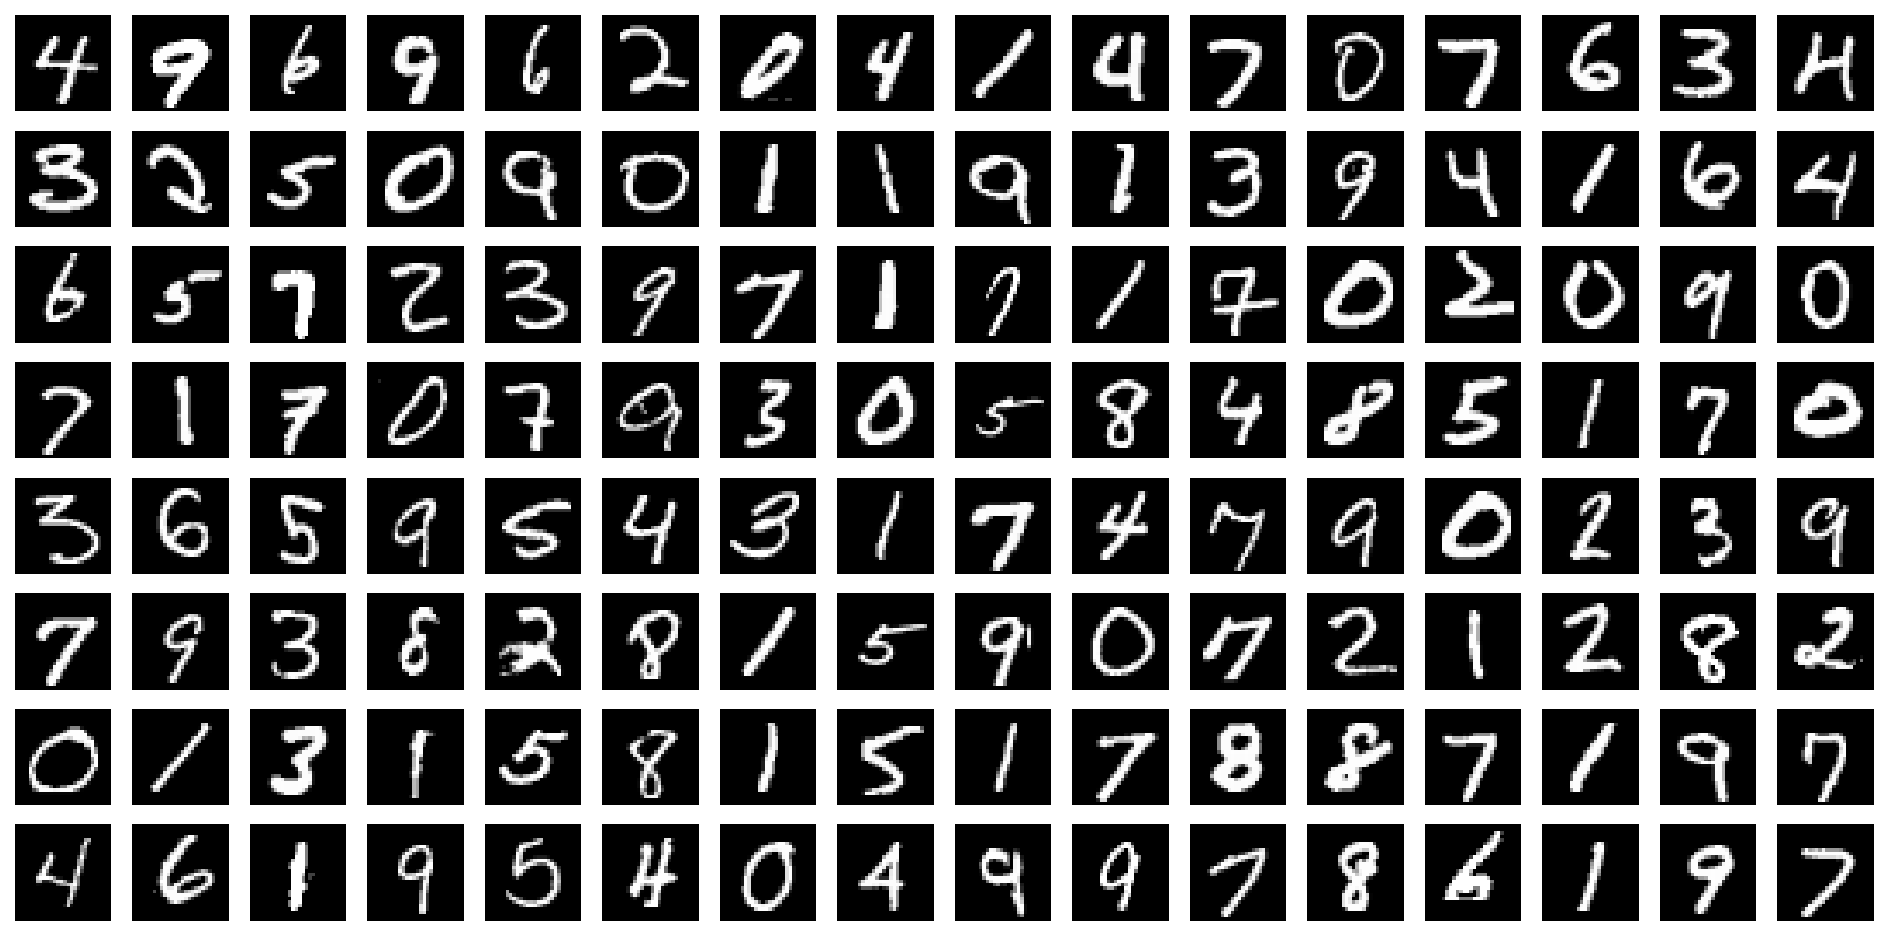
\includegraphics[width=\textwidth]{figures/mnist_random_grid_view.pdf}
\caption{MNIST数据集随机选取的$8\times 16$个样本构成的网格图}
\label{fig:mnist_random_grid_view}
\end{figure}

MNIST是非常经典的机器学习数据集,经常用作测试机器学习模型,特别是深度学习模型分类效果的基准数据集。尽管随着深度学习的发展,MNIST数据集由于规模偏小,已经不适用于评测计算机视觉领域的大模型,特别是近年来涌现的Vision Transformer\cite{dosovitskiy2021_vit},逐渐被ImageNet\cite{deng2009imagenet}, JFT-300M\cite{Sun_2017_JFT-300M}等大型数据集所取代,但经过合适处理\cite{mcmahan2017fed_avg,sahu2018fedprox}的MNIST数据集,作为联邦学习,特别是跨设备 (Cross-Silo) 场景的联邦学习的算法评测基准数据集,仍然是非常合适以及常用的\cite{reddi2020fed_opt, tran2021feddr, Ghosh_2022_cfl, li2021pfedmac, t2020pfedme}。

EMNIST数据集 (Extended MNIST database)\cite{cohen2017emnist} 是MNIST数据集的一个扩展,添加了手写的有大小写之分的26个英文字母图片,共计62类。EMNIST数据集也是常用的联邦学习的算法评测基准数据集\cite{sahu2018fedprox, zhang2020fedpd, acar2021feddyn}。数据集MNIST和EMNIST都来源于美国国家标准技术研究所 (National Institute of Standards and Technology, NIST)的手写表格和字符数据库 (Handprinted Forms and Characters Database)\cite{nist-19}。

本文实现的联邦学习仿真系统\texttt{fl-sim}在\texttt{data\_processing}模块收录的MNIST/EMNIST相关的联邦数据集有
\begin{itemize}
    \item \texttt{FedMNIST}:(依照参考文献\parencite{sahu2018fedprox}的处理方式,并基于FedML\cite{he_2020_fedml}的实现) 将数据分为1000份 (1000个子节点),每份数据只有2类手写数字,每份数据的样本量的分布遵循幂律 (Power Law)。
    \item \texttt{FedEMNIST}:(依照参考文献\parencite[附录C.2]{reddi2020fed_opt}的处理方式,并基于FedML\cite{he_2020_fedml}的实现) 将数据集按书写者分为3400份 (3400个子节点)。
    \item \texttt{FedProxFEMNIST}:(依照参考文献\parencite{sahu2018fedprox}特殊处理过的EMNIST数据集的子集) 选取EMNIST数据集中的10类 (手写的小写英文字母``a''--``j'') 随机分为200份 (200个子节点),每一份数据只包含10个类别中的5类。
    \item \texttt{FedRotatedMNIST}:(依照参考文献\parencite{Ghosh_2022_cfl}特殊处理的MNIST数据集) 将每幅图片旋转多个角度 (例如$0^\circ, 90^\circ, 180^\circ, 270^\circ$),并将数据平均分配成多份 (多个子节点),保证每一份数据上图片旋转的角度一致 (例如都旋转了$90^\circ$)。这样一来,参与联邦学习训练的节点自然形成了多个聚落 (Cluster),非常适合用于评测聚类联邦学习相关的算法。
\end{itemize}

CIFAR10/100数据集\cite{cifar}由抓取自互联网并统一降采样为$32\times 32$像素大小的RGB~3通道图片组成,共有60000张图片,分为10/100类,以作者的工作单位加拿大高等研究所 (Canadian Institute for Advanced Research) 命名。图\ref{fig:cifar10_random_grid_view}~是从CIFAR10数据集中随机抽取$8\times 16$张图片组成的网格图。CIFAR10/100也是目前联邦学习理论及算法研究中最常用的基准数据集之一\cite{zhang2020fedpd,acar2021feddyn,Ghosh_2022_cfl}。

\begin{figure}[ht]
\centering
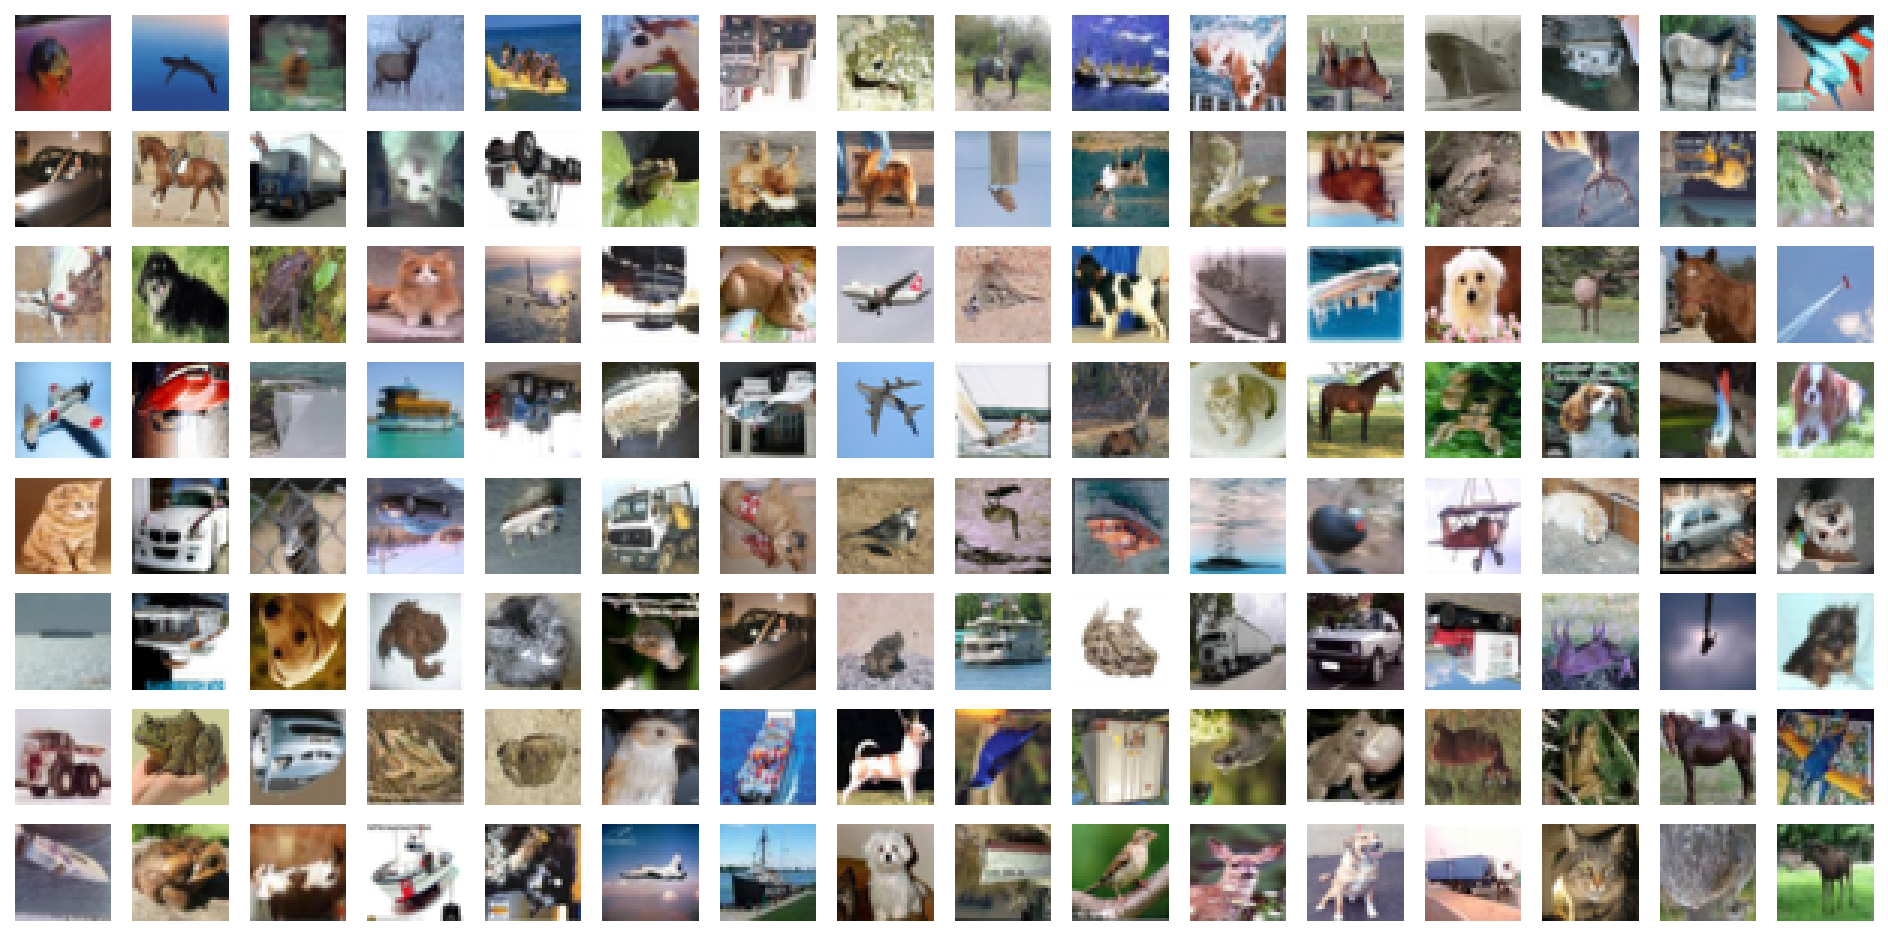
\includegraphics[width=\textwidth]{figures/cifar10_random_grid_view.pdf}
\caption{CIFAR10数据集随机选取的$8\times 16$个样本构成的网格图}
\label{fig:cifar10_random_grid_view}
\end{figure}

本文实现的联邦学习仿真系统\texttt{fl-sim}在\texttt{data\_processing}模块收录的CIFAR10/100相关的联邦数据集有
\begin{itemize}
    \item \texttt{FedCIFAR100}:(依照TensorFlow Federated\footnote{\url{https://www.tensorflow.org/federated}}的处理方式,并基于FedML\cite{he_2020_fedml}的实现) 基于CIFAR100数据集的粗标签 (Coarse Label) 以及细标签 (Fine Label) 这一两层的标签结构,利用两层的隐狄利克雷分布 (Latent Dirichlet Allocation, LDA) \index{隐狄利克雷分布, Latent Dirichlet Allocation, LDA}\cite{Li_2006_LDA}将50000张训练集的图像均分为500份 (500个子节点)。类似地,10000张训练集的图像被平均分配到了前100个子节点上。值得注意的是,在这种分配方式下,并不是所有子节点上都有测试数据。
    \item \texttt{FedRotatedCIFAR10}:生成方式与\texttt{FedRotatedMNIST}\cite{Ghosh_2022_cfl}类似,不同之处在于基础数据集从MNIST替换为了CIFAR10。
\end{itemize}

Shakespeare  待写。。。

Sent140  待写。。。

Synthetic  待写。。。

% \begin{figure}[H]
% \centering
% 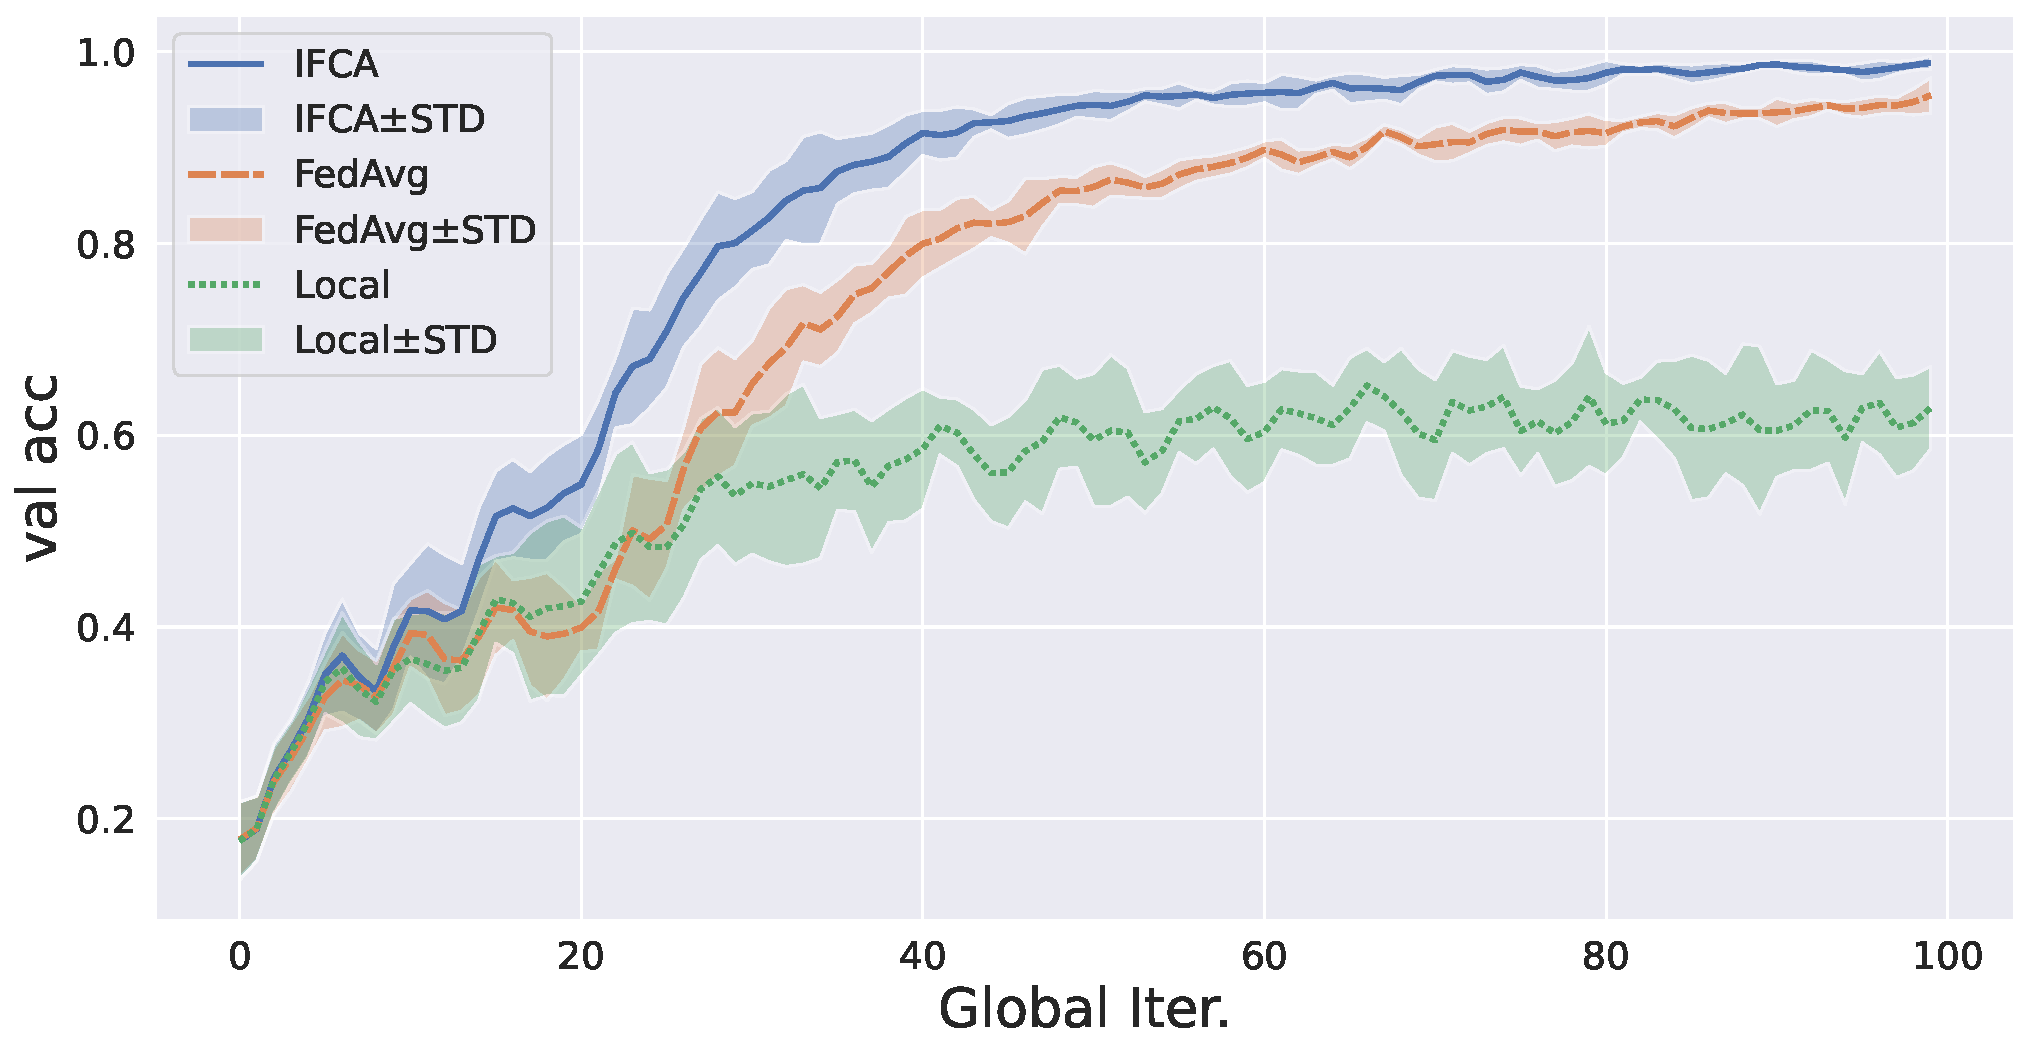
\includegraphics[width=\textwidth]{figures/fedproxfemnist.pdf}
% \caption{待写}
% \label{fig:fedproxfemnist-experiment}
% \end{figure}

待写。。。。
